\chapter{Results}\label{chap:results}

We have implemented this method both as standalone and as a~plugin for a~real-time planet renderer as we already mentioned in the~introduction. We did so in order to evaluate the~usability of the~method in practice on real data. With this method used by the~renderer, we compressed and then real-time viewed the~whole-Earth height data with 90~m span between height samples (SRTM\footnote{http://www2.jpl.nasa.gov/srtm/}~\cite{srtm}). The~total size of this dataset is 58~GB. Due to the~data redundancy of the~LOD hierarchy of the~renderer which is caused by the~fact that it stores all LODs of terrain completely separately, the~total size of the~SRTM dataset converted to this hierarchy was 260~GB. When we applied this compression method to every independent square node of this LOD hierarchy, we managed to compress these data down to 7~GB with the~maximum deviation of the~compression set to 5~m. This yields the~compression ratio of 37:1.

For a~comparison, C-BDAM~\cite{cbdam} achieved the~compression ratio of 64:1 on the~same 90~m-resolution SRTM dataset with no redundancy with the~maximum error bound set to 16~m. As we already mentioned, C-BDAM contains its own LOD rendering hierarchy without any redundancy --- a~finer LOD is constructed from the~coarser one which is where the~compression takes place. Thanks to this, there is no data redundancy in the~LOD hierarchy of C-BDAM, so the~compression ratio of this method was evaluated with respect to the~original size of the~dataset which is 58~GB. The~final size of the~compressed data prepared for rendering in C-BDAM was just 870~MB.

The~most accurate comparison of our method with C-BDAM we could perform was compress the~SRTM dataset prepared for rendering in the~mentioned application by our method with the~maximum deviation set to 16~m. We did so, the~final size of the~data was ???~GB which yield the~compression ratio of ??? when compared to the~size of the~dataset prepared for the~renderer (260~GB). However, in terms of functionality, C-BDAM is not analogic to our method, because our method cannot handle the~rendering. It is only analogic to the~renderer with our method plugged in --- only this way, both compression and rendering are achieved.

Fig.~\ref{fig:result_samples} shows a~part of a~heightmap compressed by this method, along with the~differences from the~original.

\newcommand{\hspaceimg}{\hspace{0.05cm}}
\newcommand{\vspaceimg}{\vspace{0.15cm}}
\newcommand{\incexamplsolo}[1]{\includegraphics[width=0.5\textwidth]{#1}}

\begin{figure}
	\begin{center}
	\incexamplsolo{figures/samp_orig.png} \\ \vspaceimg
	\incexamplsolo{figures/samp_comp.png} \\ \vspaceimg
	\incexamplsolo{figures/samp_diff.png}
	\end{center}
	\caption{From the~top to the~bottom --- the~original terrain, the~same terrain compressed with the~maximum deviation of 5m, the~difference between these~two. The~brighter the~color, the~greater the~value. In the~difference image, the~yellow color means 4.5m, whereas the~blue color means -4.5m.}
	\label{fig:result_samples}
\end{figure}

\newcommand{\incexamplpair}[1]{\includegraphics[width=0.45\textwidth]{#1}}

\begin{figure}
	\begin{center}
	\incexamplpair{figures/dim_64_amp_16_lon_4_horizontal_orig.png} \hspaceimg
	\incexamplpair{figures/dim_64_amp_16_lon_16_horizontal_orig.png} \\ \vspaceimg
	\incexamplpair{figures/dim_64_amp_16_lon_4_horizontal_out.png} \hspaceimg
	\incexamplpair{figures/dim_64_amp_16_lon_16_horizontal_out.png} \\ \vspaceimg
	\incexamplpair{figures/dim_64_amp_16_lon_4_horizontal_diff.png} \hspaceimg
	\incexamplpair{figures/dim_64_amp_16_lon_16_horizontal_diff.png}
    \end{center}
	\caption{Two synthetic test images of size 64x64, each one containing spiky terrain with the~heights ranging from -16 to 16. On the~left, the~longitude of spikes is 4, on the~right, it is 16. From the~top to the~bottom --- the~original, compressed with the~maximum deviation of 5, the~difference between these~two. The~brighter the~color, the~greater the~value. In the~difference image, the~yellow color means 4.5, whereas the~blue color means -4.5.}
	\label{fig:result_wave_samples}
\end{figure}

\section{The~compression artifacts}\label{sec:artifs}

This section is dedicated to analyzing the~artifacts visible in the~terrain compressed by this method. We will give some grayscale example visualisations of how they look, explain why they usually occur and discuss various ways how they can be reduced.

Because this method is designed with the~maximum height error as the~only measurement of quality of the~compressed data, we cannot guarantee that the~resulting terrain will look smooth and will not contain any sharp peaks within the~maximum-error bound. Due to the~character of the~method, such artifacts indeed occur. They cannot be completely avoided but we can reduce them by a~suitable choice of the~prediction filters, setting a~lower maximum deviation or by applying the~median filter to the~output of the~decompression if it is not a~problem for any reason (eg. decreased performance or increased maximum deviation).

As we already explained in Section~\ref{sec:top-down}, we use Neville interpolating filter of order 2 for all pixels, both near the~mip-map edges and in its interior. We also mentioned that C-BDAM only uses the~order 2 filter for the~pixels near the~borders and the~order 4 filter (Fig.~\ref{fig:order4}) for the~rest of them. We tried using the~order 4 filter with various weights settings for the~interior values, too. This slightly increased the~compression ratio --- probably because this~filter is better at predicting hills and valleys (Fig.~\ref{fig:order4_hills}) --- but worsened the~quality of compression by producing more significant artifacts. The~most probable cause of this is that the~order 4 filter is more sensitive to terrain changes --- it scans larger area to capture the~trends in terrain. We have found some general situations in which the~artifacts are particularly disturbing --- near smooth terrain's borders (Fig.~\ref{fig:artifs_border}) and near sharp terrain transitions (Fig.~\ref{fig:artifs_sharp_change}). 

\newcommand{\vcentered}[1]{\begingroup\setbox0=\hbox{#1}\parbox{\wd0}{\box0}\endgroup}

\newcommand{\artifWidth}{160}
\newcommand{\artifHeight}{120}
\newcommand{\incimg}[3]{\includegraphics[width=#1px, height=#2px]{#3}}
\newcommand{\incimgvcenter}[3]{\vcentered{\incimg{#1}{#2}{#3}}}
\newcommand{\incartifborder}[1]{\incimgvcenter{\artifWidth}{\artifHeight}{#1}}
\newcommand{\hspacehead}{\hspace{0.4cm}}

\begin{figure}
	\begin{center}
	Original\hspacehead\incartifborder{figures/artif_orig0.png} \hspaceimg
	\incartifborder{figures/artif_orig1.png} \\ \vspaceimg 
	Order 2\hspacehead\incartifborder{figures/artif_four0.png} \hspaceimg
	\incartifborder{figures/artif_four1.png} \\ \vspaceimg
	Order 4\hspacehead\incartifborder{figures/artif_twelve0.png} \hspaceimg
	\incartifborder{figures/artif_twelve1.png} \\ \vspaceimg
	\end{center}
	\caption{Two synthetic examples of the~difference between artifacts caused by order 2 and order 4 filters near smooth terrain's border --- in the~first row there are the~target heightmaps, in the~second, there are the~same heightmaps compressed using the~order 2 filter, in the~third row, the~heightmaps compressed with the~order 4 filter.}
	\label{fig:artifs_border}
\end{figure}

\newcommand{\incartifchange}[1]{\incimgvcenter{\artifWidth}{\artifWidth}{#1}}

\begin{figure}
	\begin{center}
	Original\hspacehead\incartifchange{figures/artif_change_orig0.png} \hspaceimg
	\incartifchange{figures/artif_change_orig1.png} \\ \vspaceimg
	Order 2\hspacehead\incartifchange{figures/artif_change_four0.png} \hspaceimg
	\incartifchange{figures/artif_change_four1.png} \\ \vspaceimg
	Order 4\hspacehead\incartifchange{figures/artif_change_twelve0.png} \hspaceimg
	\incartifchange{figures/artif_change_twelve1.png} \\ \vspaceimg
	\end{center}
	\caption{Two synthetic examples of the~difference between artifacts caused by order 2 and order 4 filters near a~sharp terrain change --- in the~first row there are the~target heightmaps, in the~second row, the~same heightmaps compressed using the~order 2 filter, in the~third row, the~heightmaps compressed with the~order 4 filter. The~span of the~values in the~original images is from 0 to 16 and the~maximum absolute deviation ($D$) of compression is set to 9.}
	\label{fig:artifs_sharp_change}
\end{figure}

Generally, the~reason why these artifacts occur is that as long as the~predictions are close enough to the~target mip-map and their quantized residuals are equal to zero, the~compressed values might remain above/under the~terrain for a~long time, but only until one prediction gets a~bit further from the~target terrain. As soon as it happens, its associated residual will be quantized to a~certain non-zero value which will result in the~reconstructed value being flipped to the~opposite side of the~real terrain which produces a~visual artifact. It is not a~coincidence that this often occurs near a~sharp change in the~terrain. The~predictions produced by the~averaging filter get a~bit different from the~adjacent ones near this change, because at these places, the~filter reaches out to the~area behind the~change (Fig.~\ref{fig:artifs_theory}). 

This difference might then cause the difference in residuals --- the~quantized residuals further from this change might be all zeroes, whereas the~residual near this change not, causing a~spike to occur. This spike will then get propagated to the~following compressed mip-map levels. The~only thing that is guaranteed is that the~maximum error bound is still satisfied. The~clipping performed by the~predicting filter near the~mip-map borders creates the~effect similar to a~sharp terrain change, too, in a~bit different way --- by the~sole fact that the~terrain behind the~border no longer follows its trend up to the~border (rising, for example), but is practically mirrored behind the~border (following the~example, falling), because instead of reaching out to the~non-existing values out of the~mip-map, the~existing ones are used.

\begin{figure}
	\includegraphics[trim={0 24cm 13cm 1cm}, clip, width=0.45\textwidth]{figures/artifs_theory.pdf}\centering
	\includegraphics[trim={0 24cm 13cm 0}, clip, width=0.45\textwidth]{figures/artifs_theory2.pdf}\centering
	\caption{Two illustrations of how artifacts can occur near sharp terrain changes --- the~black dots stand for the~predictions which are still within the~maximum-error bound $D$ from the~target terrain, the~blue dots represent the~predictions which are just slightly further from the~terrain, because their filters span to the~area behind the~change. Due to the~fact that a~uniform quantizer with the~step of $2D-1$ is applied to the~residuals, the~residuals added to the~blue predictions will cause them to be shifted by $2D - 1$ to the~top (the~image on the~left) or to the~bottom (the~image on the~right), creating sharp peaks in the~reconstructed values --- the~artifacts.}
	\label{fig:artifs_theory}
\end{figure}

We also tried to apply progressive quantization to the~residuals in order to reduce the~ artifacts in the~reconstructed terrain. In Sec.~\ref{sec:wavelets}, we mentioned that progressive quantization degrades the~coarser residuals less than the~finer (more detailed) ones. In our context, it would mean that the~maximum error of $\objdot{L}{i}$ (the~reconstructed data) equal to the~quantization interval of $\objdot{E}{i}$ (the~quantized residuals) would grow with $i$ up to $D$ at the~finest level. To compute $D_i$ --- the~maximum error of $\objdot{L}{i}$, we used the~following equation: $D_i = D * (\frac{i}{n})^k$, where $k$, a~natural number, is a~parameter of this approach. The~larger it is, the~less degraded are the~coarser levels, but the~maximum deviation of the~finer one is still $D$.

However, more careful decimation of coarser high-pass information only helps reduce large-scale artifacts which is not the~case of our artifacts --- they are mainly caused by differences between neighboring pixels which happens due to the~fact that the~residuals are cropped to respect the~maximum deviation. Indeed, our experiments with progressive quantization did not help reduce the~artifacts at all --- progressive quantization does not tackle the~problem described in the~previous paragraph. Quite to the~contrary, it makes the~artifacts in the~finest level more regularly distributed which is a~bit more disturbing. This is probably because there is less variance in deviation propagated from the~coarser levels which exposes the~regularity of the~prediction filters inside the~finest level more (Fig.~\ref{fig:artifs_progressive}). Additionally, the~progressive quantization increased the~size of data.

\newcommand{\progDim}{180}
\newcommand{\incartifprog}[1]{\incimgvcenter{\progDim}{\progDim}{#1}}
\newcommand{\vspacehead}{\vspace{0.07cm}}

\begin{figure}
	\begin{center}
		Original \\ \vspacehead
		\incartifprog{figures/pq/orig.png} \\ \vspaceimg
		Even quantization \\ \vspacehead
		\incartifprog{figures/pq/even.png} \hspaceimg
		\incartifprog{figures/pq/even_diff.png} \\ \vspaceimg
		Progressive quantization \\ \vspacehead
		\incartifprog{figures/pq/prog.png} \hspaceimg
		\incartifprog{figures/pq/prog_diff.png} \\ \vspaceimg
	\end{center}
	\caption{Comparison of artifacts at the~finest mip-map level produced by the~even quantization (as described in Chap.~\ref{chap:details}) and those produced by the~progressive quantization with $k$ set to 5, both with 10~m max. error at the~finest level. On the~top there is the~original, in the~remaining two rows there are the~compressed versions on the~left and their differences with the~original on the~right, in which the~yellow color means 9.5m and the~blue color means -9.5m.}
	\label{fig:artifs_progressive}
\end{figure}

Finally, we found only one way how to smoothen the~artifacts --- to post-process the~decompressed data. This post-processing does not happen during the~compression, but after the~decompression. In the~image processing, the~median filter~\cite{image_proc} is very suitable for "salt and pepper" noise reduction, whereas our artifacts often resemble this kind of noise (the bottom of Fig.~\ref{fig:result_samples}). This filter substitutes the~height of each pixel with the~median of its height together with the~heights of all its neighbors. The~size of the~neighborhood can vary, but we used the~simplest alternative --- 1, so that the~median of nine values is calculated (Fig.~\ref{fig:median}). However, generally, this filter can increase the~maximum deviation of the~decompressed data by any amount. For example, imagine a~very high pixel surrounded by very low pixels. In this extreme case, the~high pixel will be aligned to the~height of one of the~lower pixels. The~higher the~pixel was before, the~larger the~deviation caused by this filter will be.

\begin{figure}
	\includegraphics[width = \textwidth]{figures/median.png}
	\captionsource{An~example of basic median filtering. The~value of the~middle pixel (255) is substituted by the~median of it together with all neighboring values (96).}{Electronics and Computer Science University of Southampton, Computer Vision Demonstration Website~\cite{median} (edited)}
	\label{fig:median}
\end{figure}

To tackle this, we introduced a~simple modification to the~median filter. Before its application, we introduce another user parameter called $D_M$. It specifies the~maximum additional deviation which the~filtering by median can introduce. It behaves basically like a~hard threshold applied to the~output of the~median filter. Once the~filter has computed the~new height of a~certain pixel, we move the~old height towards it by at most $D_M$. Even with this constraint did we manage to significantly reduce the~artifacts (Fig.~\ref{fig:artifs_median}). However, filtering by median is quite an~expensive operation and as we mentioned, it is applied after the~decompression. Because the~decompression is performed in the~real-time when the~method is used inside a~renderer, and so it should be as fast as possible, we did not apply the~filtering in that case.

\begin{figure}
	\begin{center}
		Original \\ \vspacehead
		\incartifprog{figures/med/orig.png} \\ \vspaceimg
		Before median \\ \vspacehead
		\incartifprog{figures/med/no_med.png} \hspaceimg
		\incartifprog{figures/med/no_med_diff.png} \\ \vspaceimg
		After median \\ \vspacehead
		\incartifprog{figures/med/med.png} \hspaceimg
		\incartifprog{figures/med/med_diff.png} \\ \vspaceimg
	\end{center}
	\caption{Comparison of artifacts at the~finest mip-map level before and after the~median filter applied. The~maximum deviation of compression $D$ is 10~m and the~maximum deviation of the~filter $D_M$ is additional 5~m. On the~top there is the~original, in the~remaining two rows there are the~results on the~left and their differences with the~original on the~right. In the~upper difference image, the~yellow color means 9.5~m and the~blue color means -9.5~m, whereas in the~lower one, the~yellow means 14.5~m and the~blue means -14.5~m.}
	\label{fig:artifs_median}
\end{figure}